\subsection{Sprachübertragung}

\subsubsection*{Übersicht}

Mit dem Einbau von synchroner Sprachübertragung wird Praxisruf um die Funktion einer Gegensprechanalge erweitert.
Um Sprachverbindungen zu anderen Zimmern aufbauen zu können, wird die Ansicht der Mobilen Applikation um einen
Bereich für die Gegensprechanalge erweitert.
In diesem Bereich sind analog zum Bereich um Benachrichtigungen zu versenden Buttons vorhanden, über welche eine
Sprachverbindung aufgebaut werden kann.
Welche Buttons in einem Client zu Verfügung stehen muss vom Praxismitarbeitenden über das Admin UI konfiguriert werden.
Die Konfiguration eines Buttons beinhaltet den Text der auf Clientseite angezeigt wird, sowie eine Liste zu welchen
Clients Sprachverbindungen aufgebaut werden sollen.

Mit der gewählten Technologie WebRTC werden die Sprachverbindungen zwischen Clients Peer to Peer aufgebaut.
Die Verbindungen werden dabei vom Client selbst initialisiert.
Damit dies möglich ist, benötigt es einen Signaling Server, welcher die einzelnen verfügbaren Clients kennt und
den Austausch der Daten die zum Verbindungsaufbau notwendig sind koordiniert.

\subsubsection*{Benutzeroberfläche}

\subsubsection{User Interface}
\begin{figure}[h]
    \centering
    \begin{minipage}[b]{0.4\textwidth}
        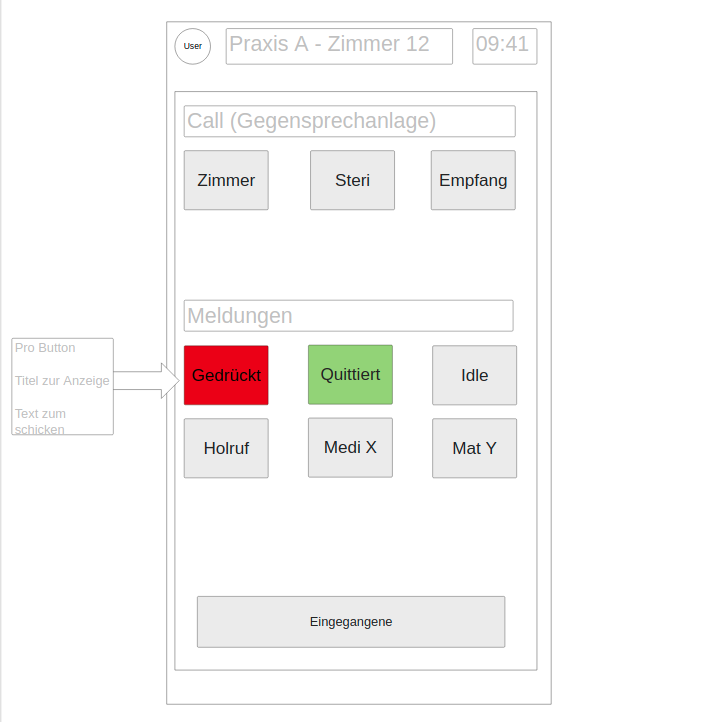
\includegraphics[width=\textwidth]{/home/joshua/FHNW/dev/IP6/IP6_Bachelorarbeit_Bericht_Cloudbasiertes_Praxisrufsystem/src/graphics/mockups/homescreen-mockup}
        \caption{Mockup Home}
    \end{minipage}
    \hfill
    \begin{minipage}[b]{0.4\textwidth}
        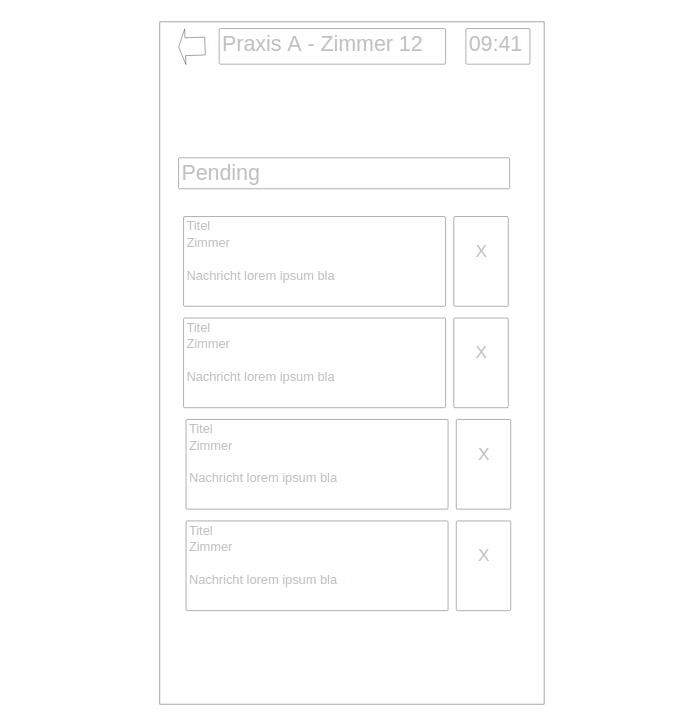
\includegraphics[width=\textwidth]{/home/joshua/FHNW/dev/IP6/IP6_Bachelorarbeit_Bericht_Cloudbasiertes_Praxisrufsystem/src/graphics/mockups/mockup-inbox}
        \caption{Mockup Inbox}
    \end{minipage}\label{fig:HomeScreen-And-Inbox-Mock}
\end{figure}

Active Call Screen \\
Erweiterung Admin UI für Konfiguration CallType \\

\clearpage
\subsubsection*{Konfiguration}

Praxisruf wird um die Funktion einer Gegensprechanlage erweitert.
Dabei soll von einem Administrator zentral konfiguriert werden können, zwischen welchen Clients Sprachverbindungen
aufgebaut werden können.
Damit dies möglich ist, sind Änderungen an der Configuration Domain des Cloud Service von Praxisruf notwendig.

Praxisruf bietet bereits heute die Möglichkeit Buttons zu konfigurieren, über welche Benachrichtigungen versendet werden können.
Diese Buttons werden mit der Entität NotificationType konfiguriert, welche wiederum einer ClientConfiguration zugeordnet werden können.
Diese ClientConfiguration wird bei der Anmeldung auf dem Mobile Client geladen und verwendet um die nötigen Buttons darzustellen.
Analog dazu wird für den Aufbau von Sprachverbindungen eine Entität CallType erstellt.
Diese kann mehreren ClientConfigurations zugeordnet werden.
Ein CallType beinhaltet den Text, welcher auf dem zugehörigen Button auf Clientseite angezeigt wird und eine Liste von
Clients, welche als Ziel der Sprachverbindung verwendet werden.
Es ist möglich, dass dieselbe Gruppe an Zielen auf verschiedenen Clients verschieden heissen soll.
Um dies einfach zu ermöglichen, werden die Ziele der Unterhaltung in eine eigene Entität CallGroup ausgelagert.
So kann pro Client ein CallType definiert werden der einen eigenen Anzeigtext definiert.
Die CallGroup muss aber nur einmal erstellt werden und kann auf mehreren CallTypes verwendet werden.
Die ClientConfiguration die bei der Anmeldung vom Mobile Client geladen wird, wird um diese CallTypes erweitert.
Dabei werden für jeden CallType aber nur der technische Identifikator und der Anzeigename mitgegeben.
Zu welchen Zielen Verbindungen aufgebaut werden sollen, wird bei jedem Verbindungsabbau erneut beim CloudService angefragt.
Dies ermögicht es, dass Änderungen an der Konfiguration sofort angewendet werden, ohne dass die ganze Konfiguration neu geladen werden muss.
Für die beiden neuen Entitäten werden Endpoints für CRUD Operationen analog zu den anderen Konfigurationsentitäten hinzugefügt.
Zudem wird das Admin UI um Ansichten erweitert, um diese Entitäten anzuzeigen, bearbeiten und löschen.

\begin{figure}[h]
    \centering
    \begin{minipage}[b]{0.7\textwidth}
        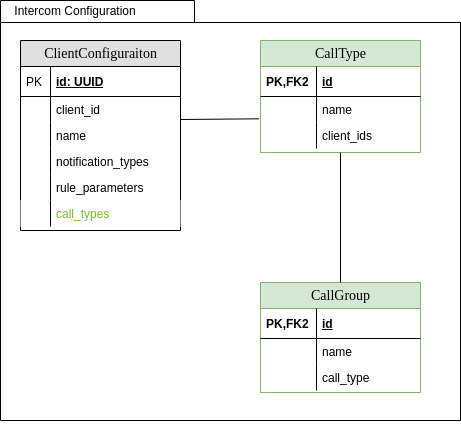
\includegraphics[width=\textwidth]{/home/joshua/FHNW/dev/IP6/IP6_Bachelorarbeit_Bericht_Cloudbasiertes_Praxisrufsystem/src/graphics/diagramms/erd_intercom_v01.drawio}
        \caption{ERD Ausschnitt - Konfiguration Gegensprechanalge}
    \end{minipage}
\end{figure}




\clearpage
\subsubsection*{Verfügbarkeit und Registrierung}

Um Sprachverbindungen zwischen Clients aufzubauen, müssen diese Nachrichten austauschen können.
Die Verbindung wird durch den Sender mit einem Offer initialisiert.
Dieses muss an den Empfänger übermittelt werden.
Dieser antwortet schliesslich mit einer Answer, welche an den Sender übermittelt werden ist.
Bevor die Verbindung aufgebaut ist, kennen die beiden Clients sich gegenseitig noch nicht.
Es braucht deshalb eine Instanz, welche beide Seiten kennt und die Übermittlung der Daten übernehmen kann.
Bei Praxisruf fällt diese Aufgabe dem Cloud Service zu.
Um dies zu ermöglichen wird Cloud Service umeine Schnittstelle erweitert, die es ermöglicht langlebige Verbindungen
zu öffnen und registrieren.
Sobald ein Client sich angemeldet hat, baut er eine Verbindung zum CloudService auf.
Beim Verbindungsaufbau gibt der Client seine technische Identifikation mit.
Der Cloud Service kann damit intern eine der verfügbaren Verbindungen und den dazugehörigen Identifikatoren führen.
Diese Liste kann beim Verbindungsaufbau verwendet werden, um die Offers und Answers an die jeweiligen Clients zu übermitteln.

Dieses Konzept wird im intercom Modul des Cloud Service umgesetzt.
Um die Funktionalität zu ermöglichen werden zwei Komponenten benötigt.
Diese kapseln die Funktionalität die unabhängig von der Technologie zum Verbindungsaufbau notwendig ist.
Um sicherzustellen, dass diese Unabhägigkeit bleibt, werden hier die Interfaces für diese beiden Komponenten spezifiziert.
Es braucht erstens eine Komponente, welche Verbindungen etabliert und Nachrichten über diese Verbindungen senden kann.
Diese Funktionalität wird mit der Komponente ClientConnector umgesetzt.

\lstinputlisting[caption=ClientConnector.java,language=java,label={lst:ClientConnector.java}]{listings/ClientConnector.java}


\clearpage
Weiter braucht es eine Komponente, welche Buch führt über bekannte Verbindungen.
Diese muss Verbindungen anhand einer id registrieren und Verbindungen wieder entfernen können.

\lstinputlisting[caption=ClientConnector.java,language=java,label={lst:ClientConnector.java}]{listings/ConnectionRegistry.java}

Der Ablauf von Anmeldung und Registrierung funktioniert damit grundsätzlich wie bisher.
Er wird aber um eine zusätzliche Registrierung über eine permanente Verbindung zum Intercom Modul ergänzt.

\begin{figure}[h]
    \centering
    \begin{minipage}[b]{0.9\textwidth}
        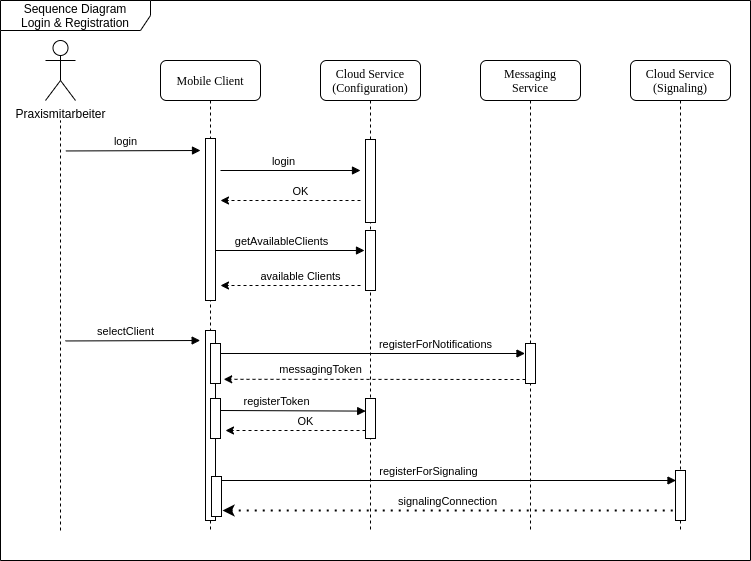
\includegraphics[width=\textwidth]{/home/joshua/FHNW/dev/IP6/IP6_Bachelorarbeit_Bericht_Cloudbasiertes_Praxisrufsystem/src/graphics/diagramms/Sequence_Registration}
        \caption{Mockup Home}
    \end{minipage}
\end{figure}


\clearpage

\subsubsection*{Verbindungsaufbau}

\begin{figure}[h]
    \centering
    \begin{minipage}[b]{0.9\textwidth}
        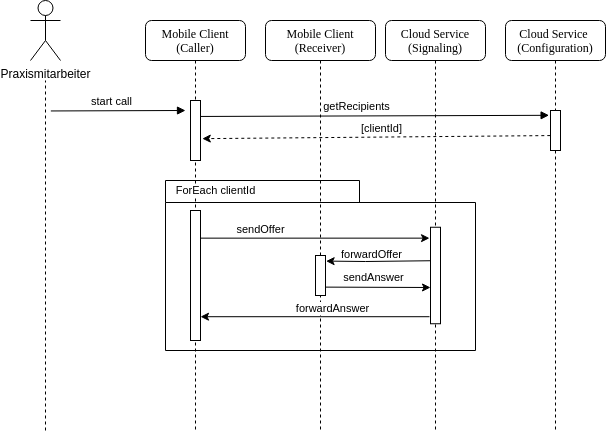
\includegraphics[width=\textwidth]{graphics/diagramms/Sequence_Intercom_Broking_V02}
        \caption{Ablauf Verbindungsaufbau Gegensprechanalge}
    \end{minipage}
\end{figure}

Wenn der Praxismitarbeitende im Mobile Client einen Button der Gegensprechanlage tippt, soll eine Sprachverbindung zu anderen Clients aufgebaut werden.
Zum Zeitpunkt an dem der Button getippt wird, weiss der Mobile Client nicht, zu welchen Clients diese Verbindung aufgebaut werden soll.
Als erstes muss deshalb beim Cloud Service angefragt werden, welche Clients mit dem betätigten Button angesprochen werden sollen.
Der Cloud Service bietet dazu einen Endpoint an über den die technischen Identifikatoren die in der CallGroup des verwendeten Buttons hinterlegt sind geladen werden.

Der Mobile Client kennt nun die technischen Identifikatoren der Clients, zu denen eine Verbindung aufgebaut werden soll.
Um die Peer To Peer Verbindung zu diesen Clients aufzubauen, müssen nun weitere Nachrichten mit dem Cloud Service ausgetauscht werden.
Alle verfügbaren Clients haben sich bei der Anmeldung mit dem Cloud Service verbunden.
Der Cloud Service führt eine Liste über die verfügbaren Verbindungen und die dazugehörigen technischen Identifikatoren.
Über diese Verbindungen werden nun die Nachrichten ausgetauscht die zum aufbauen der WebRTC Verbindung benötigt werden.
Der Austausch dieser Nachrichten folgt dem Interactive Connection Establishment Protokoll (ICE).
Der Client initialisiert für jede der erhaltenen client Ids einen Rtc Connection.
Dies dient als Endpunkt der Connection auf seiner Seite.
Anschliessend Sendet der Client ein Anfrage an den Cloud Service.
Dieses Anfrage beinhaltet das ICE Offer und die Client Ids des von Ausgangs- und Ziel-Client.
Der Cloud Service findet die Verbindung des Zieles anhand der Client Id und leitet das ICE Offer und Ausgangs Client Id über die registrierte Verbindung an den Empfänger weiter.
Wenn der Empfänger das ICE Offer erhält, initialisiert er auf seiner Seite die Rtc Connection und sendet eine Anfrage mit ICE Antwort und originaler Ausgangs Client Id an den Server zurück.
Dieser leitet die Anfrage dann analog dem ICE Offer an die Verbindung des ausgehenden Clients weiter.
Sobald dieser die Antwort erhält, ist die Rtc Connection bestätigt und die Sprachverbindung ist initialisiert.

\clearpage


\subsubsection*{Unterhaltung}

Mute Button
End Call Button


\subsubsection*{Verbindungsende}

Caller nimmt Finger vom Button.
Receiver hat button zum abbrechen.

\clearpage
